%
% magnetostatik.tex -- Herleitung Amperesches Gesetz über E-O-DGL
%
% (c) 2020 Prof Dr Andreas Müller, Hochschule Rapperswil
%
% !TEX root = ../../buch.tex
% !TEX encoding = UTF-8
%
\section{Magnetostatik\label{maxwell:magnetostatik}}
\rhead{Magnetostatik}


Wenn sich eine Ladung mit konstanter Geschwindigkeit bewegt, entsteht um sie herum ein rotationssymmetrisches Magnetfeld. Darüber hinaus wirken auch magnetische Kräfte auf die Ladung.
Wenn sich viele Ladungen mit einer konstanten Geschwindigkeit durch einen Leiter bewegen, erzeugen diese einen konstanten Strom, welcher ein zeitunabhängiges magnetisches Feld zur Folge hat. Dieses wirkt konzentrisch um den Leiter, wie in Abbildung \ref{maxwell:flussdichte} ersichtlich ist. Ausserdem ist in der Abbildung ersichtlich, dass die Feldlinien einen geschlossenen Pfad bilden. Dies zeigt, dass das magnetische Feld keine Quellen aufweist, also quellenfrei ist, und dass es somit keine magnetischen Monopole gibt.

In der Magnetostatik betrachten wir also stationäre magnetische Felder, die Ursache dafür sind Permanentmagnete oder wie bereits erwähnt Gleichströme bzw. Ladungen mit konstanter Geschwindigkeit.
Wir setzen also neu
\[ 
\frac{\partial q}{\partial t}
=
I
=
\text{const}
\]
voraus.
Zusätzlich konzentrieren wir uns in diesem Abschnitt ausschliesslich auf das magnetische Feld bzw. die magnetische Flussdichte, also nur magnetische Phänomene, somit wird auch
\[\varphi(x,y,z) = 0 \qquad \forall x,y,z\, ,\] 
also das elektrische Potentialfeld im gesamten Raum als null angenommen. 



\begin{figure}
\centering
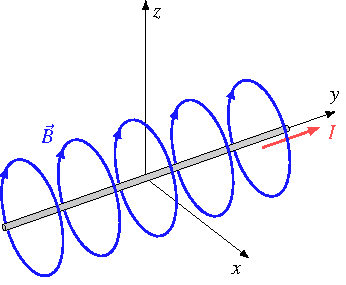
\includegraphics{papers/maxwell/images/mfeld.pdf}
% WIRE B FIELD 3D
	\caption{Magnetische Flussdichte um einen geraden Leiter}
	\label{maxwell:flussdichte}
\end{figure}




\subsubsection{Magnetisches Vektorpotential}

Wie in der Elektrostatik, gibt es auch in der Magnetostatik ein Potential, mit welchem energetische Zustände berechnet und ausgedrückt werden können. Im Unterschied ist jedoch das magnetische Potential ebenfalls eine vektorielle Grösse, also auch ein Vektorfeld. Das magnetische Vektorpotential zeigt jeweils in die selbe Richtung wie der Geschwindigkeitsvektor der bewegten Ladung.
Durch das magnetische Vektorpotential, kann die magnetische Flussdichte als 
\begin{equation}
	\operatorname{rot}\vec{A}=\nabla \times \vec{A}
	=
	\vec{B}
	\label{maxwell:definitionVektorpot}
\end{equation}
beschrieben werden, wobei wir dies für später bereits konkret ausrechnen wollen 
\begin{equation}
	\label{maxwell:nablaA}
	\renewcommand{\arraystretch}{1.9}
	\begin{pmatrix}
		\displaystyle
		\frac{\partial}{\partial x} \\
		\displaystyle
		\frac{\partial}{\partial y} \\
		\displaystyle
		\frac{\partial}{\partial z}
	\end{pmatrix}
	\times
	\begin{pmatrix}
		\displaystyle
		A_1 \\
		A_2 \\
		A_3 \\
	\end{pmatrix}
	=
	\begin{pmatrix}
		\displaystyle
		\frac{\partial A_3}{\partial y} -\frac{\partial A_2}{\partial z}\\
		\displaystyle
		\frac{\partial A_1}{\partial z} -\frac{\partial A_3}{\partial x}\\
		\displaystyle
		\frac{\partial A_2}{\partial x} -\frac{\partial A_1}{\partial y}
	\end{pmatrix}.
\end{equation}
Im Gegensatz zum elektrischen Feld, ist das magnetische Feld also kein Gradientenfeld seines Potentials, sondern ein Rotationsfeld.

Analog zur Elektrostatik, lässt sich mit dem magnetischen Vektorpotential die potentielle Energie der Wirkgrösse berechnen. Die Wirkgrösse ist jetzt allerdings keine ruhende Ladung $q$ mehr, sondern eine Ladung $q$ mit einer Geschwindigkeit $\vec{v}$, also eine bewegte Ladung. Explizit lässt sich die potentielle Energie als 
\[ W_{\text{p}} =  q\vec{v}\cdot\vec{A}\]
berechnen. Also das Skalarprodukt der Wirkgrösse und dem Potential des wirkenden Feldes an jenem Punkt im Raum.


%Mit dem Vektorpotential können ähnlich wie beim elektrischen Potential, energetische Zustände beschrieben werden. Die Wirkgrösse hier ist allerdings eine bewegte Ladung also eine Ladung $q$, welche eine Geschwindigkeit $\vec{v}$ hat. So kann das magnetische Potential dieser Grösse an einem Punkt berechnet werden. Zusätzlich ergibt sich über das Vektorpotential so auch die potentielle Energie dieser Wirkgrösse, auf welche weiter unten noch spezifischer eingegangen wird.


\subsection{Ampèresches Gesetz}
Das Ziel dieses Abschnitts ist erneut eine partielle Differentialgleichung zu finden, welche das Wesen des magnetischen Vektorpotentials und somit des magnetischen Feldes beschreibt.
Wiederum betrachten wir unter den oben vorausgesetzten Bedingungen einen luftleeren, dreidimensionalen Raum $V \subset \mathbb{R}^3$ in welchem das Vektorfeld des magnetischen Vektorpotentials $\vec{A}(x,y,z)$, somit das magnetische Feld $\vec{B}(x,y,z)$ und eine magnetische Wirkgrösse $q\vec{v}$  existieren. 

\subsubsection{Ansatz}

Wieder soll die Energie des gesamten Systems zusammengetragen und minimiert werden. 
Die Energiedichte des magnetischen Feldes mit \eqref{maxwell:definitionVektorpot} eingesetzt ist
\[ w_{\text{m}} 
= 
\frac{1}{2\mu_0}\vec{B}(x,y,z)^2
=
\frac{1}{2\mu_0}\left(\nabla\times\vec{A}(x,y,z)\right)^2. \]
Die Gesamtenergie jenes Feldes berechnet sich dann durch Integration über den gesamten Raum $V$ als
\begin{equation}
	\label{maxwell:magnetFeldEnergie}
	W_{\text{m}} = \iiint_V w_m\, dV\,.
\end{equation}
Wie bereits erwähnt, ergibt sich durch eine bewegte Ladung $q$ mit einer Geschwindigkeit $\vec{v}$ eine weitere potentielle Energie im System, welche sich als 
\[ 
W_{\text{p}}
= 
q\vec{v}
\cdot
\vec{A}
 \]
berechnen lässt.
Da unser Ziel jedoch ist, das Integral der Gesamtenergie zu minimieren, müssen wir auch diese potentielle Energie über den gesamten Raum bzw. das selbe Volumen integrieren wie das Integral in \eqref{maxwell:magnetFeldEnergie}. 

Dafür betrachten wir erneut nur ein kleines, ein infinitesimales Stück der Ladung also $dq\,\vec{v}$ und können mithilfe von $dq = \varrho\,dV$, wobei $\varrho$ die Ladungsdichte ist, dieses kleine Stück der Ladung sofort zu $\vec{v}\varrho\,dV$ umschreiben.
Wenn wir uns jetzt überlegen, dass sich eine Ladungsdichte mit einer Geschwindigkeit $\vec{v}$ bewegt, können wir auch sagen, dass dies äquivalent zu einer Stromdichte $\vec{\jmath}=\varrho\vec{v}$ ist. 
Die kleinen bzw. infinitesimalen Stücke der Wirkgrösse formen wir also zu \[\vec{\jmath}\,dV = \varrho\vec{v}\,dV\]
um und erhalten mit einer Integration über den ganzen Raum $V$
\begin{equation}
	W_{\text{p}}
	= 
	\iiint_V \vec{A}\cdot\varrho\vec{v}\,dV
	=
	\iiint_V \vec{A}(x,y,z)\cdot\vec{j}(x,y,z)\,dV
\end{equation}
die gesamte potentielle Energie der Wirkgrösse.

Jetzt befinden sich beide Energiekomponenten in einer Form, in welcher wir über denselben Raum bzw. dasselbe Volumen integrieren können und somit lassen sie sich zu einem einzigen Integral als 
\begin{align*}
W_{\text{tot}} 
&=
W_{\text{p}} - W_{\text{m}}
=
\iiint_V \vec{A}\cdot\vec{\jmath}
- \frac{1}{2\mu_0}\left(\nabla\times\vec{A}\right)\cdot\left(\nabla\times\vec{A}\right)\, dV \\
&=
\iiint_V \left( A_1j_1 + A_2j_2 + A_3j_3\right) - 
 \frac{1}{2\mu_0}\biggl( 
 	\biggl( \frac{\partial A_3}{\partial y} -\frac{\partial A_2}{\partial z}\biggr)^2 
 + \biggl( \frac{\partial A_1}{\partial z} -\frac{\partial A_3}{\partial x}\biggr)^2
 + \biggl(\frac{\partial A_2}{\partial x} -\frac{\partial A_1}{\partial y} \biggr)^2   
 \biggr) \,dV
\end{align*}
zusammenfassen.

In dieser Gleichung wird sofort das zu minimierende Integral ersichtlich und die Lagrange-Funktion kann als 

	%\begin{align}
	%\label{maxwell:magnetostatikLagrange}
	%L\left(x,y,z, \vec{A}, \vec{A}_x. \vec{A}_y, \vec{A}_z\right)
	%=&\left( A_1j_1 + A_2j_2 + A_3j_3\right) \\ \nonumber
	% &- \frac{1}{2\mu_0}\left( 
	%\left( \frac{\partial A_3}{\partial y} -\frac{\partial A_2}{\partial %z}\right)^2 
	%+ \left( \frac{\partial A_1}{\partial z} -\frac{\partial A_3}{\partial x}\right)^2
	%+ \left(\frac{\partial A_2}{\partial x} -\frac{\partial A_1}{\partial y} \right)^2   
	%\right)	
	%\end{align}
	
	\begin{align}
	\label{maxwell:magnetostatikLagrange}
	L\left(x,y,z, \vec{A}, \vec{A}_x. \vec{A}_y, \vec{A}_z\right)
	=&\left( A_1j_1 + A_2j_2 + A_3j_3\right) \\ \nonumber
	 &- \frac{1}{2\mu_0}\bigl( 
	( A_{3,y} - A_{2,z})^2 
	+ (A_{1,z} -A_{3,x})^2
	+ (A_{2,x} -A_{1,y})^2   
	\bigr)
	\end{align}
abgelesen und definiert werden. 
Hierbei wollen wir darauf hinweisen, dass die Lagrange-Funktion in diesem Fall von einem Vektor, dem magnetischen Vektorpotential $\vec{A}$ abhängig ist. 
Das bedeutet, dass jede Komponente des Vektorpotentials einzeln variiert werden kann, was später die Ursache für mehrere Ausführungen der Euler-Ostrogradski-Differentialgleichung sein wird.

Erneut stellen wir auch fest, dass ein additiver Term dazugekommen ist, wie weiter oben beschrieben handelt es sich auch um einen Kopplungsterm, welcher hier jedoch die Wechselwirkung zwischen dem Feld $\vec{A}$ und der Wirkgrösse, also der Stromdichte $\vec{\jmath}\,$ beschreibt.

\subsubsection{Einsetzen in die Euler-Ostrogradski-Differentialgleichung}

Da jede Komponente des magnetischen Vektorpotentials für sich variiert werden kann, resultieren demnach drei Euler-Ostrogradski-Differentialgleichungen der Form
\[ 
\frac{\partial L}{\partial A_i} 
- \frac{\partial}{\partial x}\frac{\partial L}{\partial A_{i,x}}
- \frac{\partial}{\partial y}\frac{\partial L}{\partial A_{i,y}}
- \frac{\partial}{\partial z}\frac{\partial L}{\partial A_{i,z}}
= 0 \qquad \text{für } i=1,2,3
\, . \]
{\larger\textcircled{\smaller[2]1}} $i = 1$:
\begin{subequations}
	\label{maxwell:magnetoL1}
\begin{gather}
	0
	=
	j_1 - \underbrace{\frac{\partial}{\partial x}\frac{\partial L}{\partial A_{1,x}}}_{=0}
	 - \left( \frac{1}{2\mu_0}(-1)\,2 \frac{\partial}{\partial y}(A_{2,x}-A_{1,y})\right) 
	 - \left( \frac{1}{2\mu_0}\,2\frac{\partial}{\partial z}(A_{1,z}-A_{3,x})\right)
	 \\
	 0
	 =
	 j_1 - \frac{1}{\mu_0}\left( \frac{\partial}{\partial y}(A_{2,x}-A_{1,y})
	 - \frac{\partial}{\partial z}(A_{1,z}-A_{3,x})
	 \right)  
	 \\	 
	 \mu_0j_1
	 =
	 \frac{\partial}{\partial y}(A_{2,x}-A_{1,y})
	 - \frac{\partial}{\partial z}(A_{1,z}-A_{3,x})	 	 	 
\end{gather}
\end{subequations}
{\larger\textcircled{\smaller[2]2}} $i = 2$:
\begin{equation}
	\label{maxwell:magnetoL2}
	\mu_0j_2
	=
	\frac{\partial}{\partial z}(A_{3,y}-A_{2,z})
	- \frac{\partial}{\partial x}(A_{2,x}-A_{1,y})
\end{equation}
{\larger\textcircled{\smaller[2]3}} $i = 3$:
\begin{equation}
	\label{maxwell:magnetoL3}
	\mu_0j_3
	=
	\frac{\partial}{\partial x}(A_{1,z}-A_{3,x})
	- \frac{\partial}{\partial y}(A_{3,y}-A_{2,z})
\end{equation}
Wobei für $i=2,3$ genau das gleiche Vorgehen wie bei $i=1$ angewendet wurde.
Mithilfe von \eqref{maxwell:nablaA} wollen wir jetzt den Ausdruck $\nabla\times\nabla\times\vec{A} = \nabla\times\vec{B}$ betrachten.

\begin{equation}
	\renewcommand{\arraystretch}{1.9}
	\begin{pmatrix}
		\displaystyle
		\frac{\partial}{\partial x} \\
		\displaystyle
		\frac{\partial}{\partial y} \\
		\displaystyle
		\frac{\partial}{\partial z}
	\end{pmatrix}
	\times
	\begin{pmatrix}
		\displaystyle
		\frac{\partial A_3}{\partial y} -\frac{\partial A_2}{\partial z}\\
		\displaystyle
		\frac{\partial A_1}{\partial z} -\frac{\partial A_3}{\partial x}\\
		\displaystyle
		\frac{\partial A_2}{\partial x} -\frac{\partial A_1}{\partial y}
	\end{pmatrix}
	=
	\begin{pmatrix}
		\displaystyle
		\frac{\partial}{\partial y}(A_{2,x}-A_{1,y}) - \frac{\partial}{\partial z}(A_{1,z}-A_{3,x})	\\
		\displaystyle
		\frac{\partial}{\partial z}(A_{3,y}-A_{2,z}) - \frac{\partial}{\partial x}(A_{2,x}-A_{1,y}) \\
		\displaystyle
		\frac{\partial}{\partial x}(A_{1,z}-A_{3,x}) - \frac{\partial}{\partial y}(A_{3,y}-A_{2,z})
	\end{pmatrix}
\end{equation}
Wir stellen fest, dass die drei Komponenten des resultierenden Vektors genau mit den rechten Seiten der drei Gleichungen \eqref{maxwell:magnetoL1}, \eqref{maxwell:magnetoL2} und \eqref{maxwell:magnetoL3} übereinstimmen.
Dank der kompakten vektoriellen Schreibweise, können wir also unser Ergebnis der genannten drei Gleichungen zu
\[ 
\mu_0\vec{\jmath} 
= 
\nabla \times \vec{B}
 \]
zusammenfassen. Hierbei resultiert das ampèresche Gesetz.

\subsubsection{Interpretation des Resultates}

Mittels der Variationsrechnung konnten wir das ampèresche Gesetz herleiten, welches besagt, dass die Stromdichte proportional zur Rotation des magnetischen Feldes ist. Anders ausgedrückt kann man auch sagen, dass die Stromdichte, welche durch eine Fläche strömt, proportional zum magnetischen Feld ist, welches um den Rand dieser selben Fläche wirkt.


